%Este trabalho está licenciado sob a Licença Atribuição-CompartilhaIgual 4.0 Internacional Creative Commons. Para visualizar uma cópia desta licença, visite http://creativecommons.org/licenses/by-sa/4.0/deed.pt_BR ou mande uma carta para Creative Commons, PO Box 1866, Mountain View, CA 94042, USA.

\chapter{Sistemas Lineares}\label{cap_sislin}

Neste capítulo, estudamos métodos numéricos para a resolução de sistemas lineares de médio e grande porte. Salvo explicitado ao contrário, assume-se que os sistemas são quadrados e têm solução única.

\section{Matrizes Esparsas}\label{cap_sislin_sec_matesparsa}

\hl{Uma matriz é dita ser \emph{esparsa} quando ela tem apenas poucos elementos não nulos}. A ideia é que os elementos não nulos não precisam ser guardados na memória do computador, gerando um grande benefício na redução da demanda de armazenamento de dados. O desafio está no desenvolvimento de estruturas de dados para a alocação eficiente de tais matrizes, i.e. que sejam suficientemente adequadas para os métodos numéricos conhecidos.

\begin{figure}[H]
  \centering
  \includegraphics[width=0.45\textwidth]{./cap_sislin/dados/matriz_esparsa_estruturada/main}\\
  \includegraphics[width=0.45\textwidth]{./cap_sislin/dados/matriz_esparsa_nao_estruturada/main}
  \caption{Em cima: exemplo de uma matriz esparsa estruturada. Em baixo: exemplo de uma matriz esparsa não-estruturada.}
  \label{fig:ex_matriz_esparsa_estrutura}
\end{figure}

\hl{Matrizes esparsas podem ser classificadas como \textbf{estruturadas} ou \textbf{não-estruturadas}}. Uma matriz estruturada é aquela em que as entradas não-nulas formam um padrão regular. Por exemplo, estão dispostas em poucas diagonais ou formam blocos (submatrizes densas) ao longo de sua diagonal principal. No caso de não haver um padrão regular das entradas não-nulas, a matriz esparsa é dita ser não-estruturada. Consulte a Figura \ref{fig:ex_matriz_esparsa_estrutura} para exemplos.

\hl{A \textbf{esparsidade} de uma matriz é a porcentagem de elementos nulos que ela tem}, i.e. para uma matriz quadrada $n\times n$ tem-se que a esparsidade é
\begin{equation}\hleq
  e := \frac{n_{\text{nulos}}}{n^2}\times 100\%.
\end{equation}
Por exemplo, a matriz identidade de tamanho $n=100$ tem esparsidade
\begin{equation}
  e = \frac{100^2 - 100}{100^2}\times 100\% = 99\% .
\end{equation}

\subsection{Sistemas Tridiagonais}

Um \hlemph{sistema tridiagonal} tem a seguinte forma matricial
\begin{equation}\label{eq:sistridiag}
  \begin{bmatrix}
    a_{1,1} & {\color{violet}a_{1,2}} & & & & 0\\
    {\color{teal}a_{2,1}} & a_{2,2} & {\color{violet}a_{2,3}} & & &\\
    & {\color{teal}a_{3,2}} & a_{3,3} & {\color{violet}a_{3,4}} & &\\
    & & \ddots & \ddots & \ddots &\\
    & & & \ddots & \ddots & {\color{violet}a_{n-1,n}}\\
    0 & & & & {\color{teal}a_{n,n-1}} & a_{n,n}
  \end{bmatrix}
  \begin{bmatrix}
    x_1\\
    x_2\\
    x_3\\
    \vdots\\
    x_{n-1}\\
    x_n
  \end{bmatrix} =
    \begin{bmatrix}
    b_1\\
    b_2\\
    b_3\\
    \vdots\\
    b_{n-1}\\
    b_n
  \end{bmatrix}.
\end{equation}
Ou seja, \hl{é um sistema cuja a matriz dos coeficientes é tridiagonal}.

\hl{Uma \emph{matriz tridiagonal} é uma matriz esparsa estruturada}. Mais especificamente, é um caso particular de uma \hlemph{matriz banda}, em que os elementos não nulos estão dispostos apenas em algumas de suas diagonais. Para armazenarmos tal matriz precisamos alocar apenas os seguintes três vetores
\begin{align}
  & {\color{violet}d_{1} = \left(0,a_{1,2},\dotsc,a_{n-1,n}\right)},\\
  & d_{0} = \left(a_{1,1},a_{2,2},\dotsc,a_{n,n}\right),\\
  & {\color{teal}d_{-1} = \left(a_{2,1},\dotsc,a_{n,n-1},0\right)}.
\end{align}
Ou seja, precisamos armazenar $3n$ pontos flutuantes em vez de $n^2$, como seria o caso se a matriz dos coeficientes fosse densa. Com isso, podemos alocar a matriz do sistema da seguinte forma
\begin{equation}
  \tilde{A} =
  \begin{bmatrix}
    {\color{violet}*} & {\color{violet}a_{1,2}} & {\color{violet}\cdots} & {\color{violet}a_{n-1,n}}\\
    a_{1,1} & a_{2,2} & \cdots & a_{n,n}\\
    {\color{teal}a_{2,1}} & {\color{teal}\dotsc} & {\color{teal}a_{n,n-1}} & {\color{teal}*}
  \end{bmatrix}.
\end{equation}
Ou seja, $\tilde{A} = [\tilde{a}_{i,j}]_{i,j=1}^{3,n}$, sendo
\begin{equation}
  \tilde{a}_{1+i-j,j} = a_{i,j}.
\end{equation}

\begin{ex}
  Seja o seguinte sistema linear
  \begin{gather}
    2x_1 - x_2 = 0\\
    x_{i-1} - 6x_i + 4x_{i+1} = \sen\left(i\frac{\pi}{2(n-1)}\right)\\
    x_{n-1} + x_n = 1
  \end{gather}
  
  O seguinte código {\python} faz a alocação de seu vetor dos termos constantes $b$ e de sua matriz de coeficientes no formato compacto de $\tilde{A}$.

\begin{lstlisting}[caption=diagSis.py, label={py:diagSis}]
import numpy as np
n = 100000

# alocação
# vetor dos termos constantes
b = np.empty(n)
b[0] = 0.
for i in range(1,n-1):
  b[i] = np.sin(i*np.pi/(2*(n-1)))
b[n-1] = 1.
print(b)
print(f"b size: {b.size*b.itemsize/1024} Kbytes")

# matriz compacta
tA = np.zeros((3,n))

# indexação
def ind(i,j):
return 1+i-j,j

tA[ind(0,0)] = 2.
tA[ind(0,1)] = -1.
for i in range(1,n-1):
  tA[ind(i,i-1)] = 1.
  tA[ind(i,i)] = -3.
  tA[ind(i,i+1)] = 4.
tA[ind(n-1,n-2)] = 1.
tA[ind(n-1,n-1)] = 1.
print(tA)
print(f"tA size: {tA.size*tA.itemsize/1024**2:1.1f} Mbytes")
\end{lstlisting}

\end{ex}

\subsubsection{Algoritmo de Thomas (TDMA)}

\hl{O \emph{algoritmo de Thomas}{\thomas} ou \emph{TDMA} (do inglês, \textit{Tridiagonal Matrix Algorithm}) é uma forma otimizada do método de eliminação gaussiana}{\gauss}\hl{ aplicada a sistemas tridiagonais}. Enquanto este requer $O(n^3)$ operações, esse demanda apenas $O(n)$.

Eliminando os termos abaixo da diagonal em \eqref{eq:sistridiag}, obtemos o sistema equivalente
\begin{equation}
  \begin{bmatrix}
    a_{1,1} & a_{1,2} & & & 0 & | & b_1\\
      & \tilde{a}_{2,2} & a_{2,3} & & & | & \tilde{b}_2\\
    &  & \tilde{a}_{3,3} & \ddots & & | & \vdots \\
    & & & \ddots & a_{n-1,n} & | & \tilde{b}_{n-1}\\
    0 & & & & \tilde{a}_{n,n} & | & \tilde{b}_n
  \end{bmatrix}
\end{equation}
Este é obtido pela seguinte iteração
\begin{align}
  & w \leftarrow \frac{a_{i+1,i}}{a_{i,i}}\\
  & a_{i,i} \leftarrow a_{i,i} - w\cdot a_{i-1,i}\\
  & b_i \leftarrow b_i - w\cdot b_{i-1}
\end{align}
onde, o {\textasciitilde} foi esquecido de propósito, indicando a reutilização da matriz $\tilde{A}$ e do vetor $b$. A solução do sistema é, então, obtida de baixo para cima, i.e.
\begin{gather}
  x_n \leftarrow \frac{b_n}{a_{n,n}}\\
  x_i \leftarrow \frac{b_i - a_{i,i+1}x_{i+1}}{a_{i,i}},
\end{gather}
com $i=n-1,n-2,\dotsc,1$.

\begin{lstlisting}[caption=tdma.py, label={py:tdma}]
def tdma(ta, b):
  a = ta.copy()
  x = b.copy()
  # eliminação
  for i in range(1,n):
    w = a[2,i-1]/a[1,i-1]
    a[1,i] -= w * a[0,i]
    x[i] -= w * x[i-1]
  # resolve
  x[n-1] = x[n-1]/a[1,n-1]
  for i in range(n-2,-1,-1):
    x[i] = (x[i] - a[0,i+1]*x[i+1])/a[1,i]
  return x
\end{lstlisting}


\subsection{Matrizes Banda}

\hl{Uma \emph{matriz banda} é aquela em que os elementos não nulos estão dispostos em apenas algumas de suas diagonais}. Consulte a Figura \ref{fig:MatrizBanda}.

\begin{figure}[H]
  \centering
  \includegraphics[width=0.45\textwidth]{./cap_sislin/dados/figMatrizBanda/main}
  \caption{Exemplo de uma matriz banda.}
  \label{fig:MatrizBanda}
\end{figure}

\begin{ex}\label{ex:poisson}
  Consideramos o seguinte problema de Poisson{\poisson}
  \begin{align}
    &- \Delta u = f(x,y),~(x, y)\in (0, \pi)\times (0, \pi),\\
    &u(0, y) = 0,~y\in [0, \pi],\\
    &u(\pi, y) = 0,~y\in [0, \pi],\\
    &u(x, 0) = 0,~x\in [0, \pi],\\
    &u(x, \pi) = 0,~x\in [0, \pi],
  \end{align}
  onde, $\Delta := \left(\frac{\p^2}{\p x^2}, \frac{\p^2}{\p y^2}\right)$ é o operador laplaciano{\laplace}. Para fixarmos as ideias, vamos assumir
  \begin{equation}
    f(x,y) = \sen(x)\sen(y)
  \end{equation}
  
  Vamos empregar o \textbf{método de diferenças finitas} para computar uma aproximação para a sua solução. Começamos assumindo uma malha uniforme de $n^2$ nodos
  \begin{align}
    & x_i = (i-1)h\\
    & y_j = (j-1)h
  \end{align}
  com tamanho de malha $h = \pi/(n-1)$, $i=1,2,\dotsc,n$ e $j=1,2,\dotsc,n$. Empregando a fórmula de diferenças central, encontramos o seguinte problema discreto associado
  \begin{align}
    &u_{i, 1} = u_{1, j} = 0\\
    &~\nonumber\\
    &- \frac{1}{h^2}u_{i-1,j} - \frac{1}{h^2}u_{i,j-1} + \frac{4}{h^2}u_{i,j} \nonumber\\
    &\qquad- \frac{1}{h^2}u_{i+1,j} - \frac{1}{h^2}u_{i,j+1} = f(x_i, y_j)\\
    &~\nonumber\\
    &u_{i,n} = u_{n,j} = 0
  \end{align}

  Este é um sistema linear $n^2 \times n^2$. Tomando em conta as condições de contorno, ele pode ser reduzido a um sistema $(n-2)^2\times (n-2)^2$
  \begin{equation}
    Aw = b
  \end{equation}
  usando a enumeração das incógnitas 
  \begin{equation}
    (i,j) \rightarrow k=i-1 + (j-2)(n-2), 
  \end{equation}
  i.e.
  \begin{equation}
    u_{i,j} = w_{k=i-1 + (j-2)(n-2)}
  \end{equation}
para $i,j=2,\dotsc,n-2$. Consulte a Figura \ref{fig:malha2d} para uma representação da enumeração em relação a malha.

  \begin{figure}[H]
    \centering
    \includegraphics[width=5in]{./cap_sislin/dados/figMalha2D/fig}
    \caption{Representação da enumeração das incógnitas referente ao problema discutido no Exemplo \ref{ex:poisson}.}
    \label{fig:malha2d}
  \end{figure}

  Afim de obtermos uma matriz diagonal dominante, vamos ordenar as equações do sistema discreto como segue
  \begin{itemize}
  \item $j=2$, $i=2$:
    \begin{equation}\label{cap_sislin_sec_matesparsa:eq:ex_poisson_deq0}
      4w_k - w_{k+1} - w_{k+n-2} = h^2f_{i,j}
    \end{equation}
  \item $j=2$, $i=3,\dotsc,n-2$:
    \begin{equation}
      -w_{k-1} + 4w_{k} - w_{k+1} - w_{k+n-2} = h^2f_{i,j}
    \end{equation}
  \item $j=2$, $i=n-1$:
    \begin{equation}
      -w_{k-1} + 4w_k - w_{k+n-2} = h^2f_{i,j}
    \end{equation}
  \item $j=3,\dotsc,n-2$, $i=2$:
    \begin{equation}
      -w_{k-(n-2)} + 4w_k - w_{k+1} - w_{k+n-2} = h^2f_{i,j}
    \end{equation}
  \item $j=3,\dotsc,n-2$, $i=3,\dotsc,n-2$:
    \begin{equation}
      -w_{k-1} - w_{k-(n-2)} + 4w_k - w_{k+1} - w_{k+n-2} = h^2f_{i,j}
    \end{equation}
  \item $j=3,\dotsc,n-2$, $i=n-1$:
    \begin{equation}
      -w_{k-1} - w_{k-(n-2)} + 4w_k - w_{k+n-2} = h^2f_{i,j} 
    \end{equation}
  \item $j=n-1$, $i=2$:
    \begin{equation}
      -w_{k-(n-2)} + 4w_k - w_{k+1} = h^2f_{i,j}
    \end{equation}
  \item $j=n-1$, $i=3,\dotsc,n-2$:
    \begin{equation}
      -w_{k-1} - w_{k-(n-2)} + 4w_k - w_{k+1} = h^2f_{i,j}
    \end{equation}
  \item $j=n-1$, $i=n-1$:
    \begin{equation}
      -w_{k-1} - w_{k-(n-2)} + 4w_k = h^2f_{i,j}\label{cap_sislin_sec_matesparsa:eq:ex_poisson_deq1}
    \end{equation}
  \end{itemize}
  Com isso, temos um sistema com matriz com 5 bandas, consulte a Figura \ref{fig:exPoissonMatriz}.

  \begin{figure}[H]
    \centering
    \includegraphics[width=0.7\textwidth]{./cap_sislin/dados/figExPoissonMatriz/fig}
    \caption{Representação da matriz do sistema discreto construído no Exemplo \ref{ex:poisson}.}
    \label{fig:exPoissonMatriz}
  \end{figure}
\end{ex}


\subsection{Esquemas de Armazenamento}

A ideia é armazenar apenas os elementos não-nulos de uma matriz esparsa, de forma a economizar a demanda de armazenamento computacional. Cuidados devem ser tomados para que a estrutura de armazenamento utilizada seja adequada para a computação das operações matriciais mais comuns.

\subsubsection{Formato COO}

O \hlemph{formato COO} (do inglês, \textit{COOrdinate format}) é o esquema de armazenamento simples de matrizes esparsas. As estrutura de dados consiste em três arranjos:
\begin{enumerate}[1.]
  \item um arranjo contendo as entradas não-nulas da matriz; 
  \item um arranjo contendo seus índices de linha; 
  \item um arranjo contendo seus índices de coluna.
\end{enumerate}
O método {\PYTHONscipyDOTsparseDOTcooArray} permite a alocação de matrizes no formato COO. 

\begin{ex}\label{ex:coo}
  O seguinte código armazena a matriz
  \begin{equation}
    A =
    \begin{bmatrix}
      2. & 0. & 1.  & 0.\\
      0. & 3. & 2.  & -1.\\
      0  & -1 & -2. & 0.\\
      0  & 0  & 0   & 1.
    \end{bmatrix}
  \end{equation}
  no formato COO.

\begin{lstlisting}
import numpy as np
from scipy.sparse import coo_array

data = np.array([2.,1.,3.,2.,-1.,-1.,-2.,1.])
row = np.array([0,0,1,1,1,2,2,3])
col = np.array([0,2,1,2,3,1,2,3])
A = coo_array((data, (row, col)), shape=(4,4))
print("A = \n", A)
print("A = \n", A.toarray())
\end{lstlisting}

\end{ex}

\begin{itemize}
\item \hl{Vantagens do formato COO} são:
  \begin{itemize}
  \item permite a entrada de dados duplicados (simplicidade);
  \item conversão rápida para os formatos CSR e CSC\endnote{CSR e CSC são formatos de matrizes esparsas mais eficientes para a computação matricial.}.
  \end{itemize}
  
\item \hl{Desavantagens do formato COO} são:
  \begin{itemize}
  \item complexidade em operações aritméticas;
  \item complexidade na extração de submatrizes.
  \end{itemize}
\end{itemize}

\begin{obs}\normalfont{(\hl{Entradas Duplicadas}.)}
  O formato COO permite a entrada duplicada de elementos da matriz. Na conversão para outros formatos (por exemplo, CSR ou CSC), as entradas duplicadas são somadas.
\end{obs}

\subsubsection{Formato CSR}
\badgeRevisar

O formato {\it Compressed Sparse Row} (CSR) é uma variação do COO que busca diminuir a alocação de dados repetidos. Assim como o COO, o formato conta com três arranjos $d$, $c$, $p$:
\begin{itemize}
\item $d$ é o arranjo contendo os elementos não-nulos da matriz, ordenados por linhas (i.e., da esquerda para direita, de cima para baixo);
\item $c$ é o arranjo contendo o índice das colunas das entradas não-nulas da matriz (como no formato COO);
\item $p$ é um arranjo cujos elementos são a posição no arranjo $c$ em que cada linha da matriz começa a ser representada. O número de elementos de $i$-ésima linha da matriz dado por $p_{j+1}-p_j$.
\end{itemize}

\begin{ex}
  No Exemplo \ref{ex:coo}, alocamos a matriz
  \begin{equation}
    A =
    \begin{bmatrix}
      2. & 0. & 1.  & 0. \\
      0. & 3. & 2.  & -1.\\
      0  & -1 & -2. & 0. \\
      0  & 0  & 0   & 1.
    \end{bmatrix}
  \end{equation}
  no formato COO. Aqui, vamos converter a alocação para o formato CSR e, então, verificar seus atributos.
  \begin{lstlisting}
    from scipy.sparse import csr_matrix
    csr = coo.tocsr()
    d = csr.data
    c = csr.indices
    p = csr.indptr
    print(d)
    print(c)
    print(p)
  \end{lstlisting}
  Para fixarmos as ideias, temos
  \begin{gather}
    d = (2., 1., 3., 2., -1., -1., -2., 1.)\\
    c = (0, 2, 1, 2, 3, 1, 2, 3)\\
    p = (0, 2, 5, 7, 8)
  \end{gather}
  Assim sendo, o elemento \lstinline+p[i=2] = 5+ aponta para o \lstinline+c[k=5] = 1+, o que fornece que \lstinline+A[i=2,j=1]=d_{k}=-1.+. Verifique!
\end{ex}

\begin{itemize}
\item Vantagens do formato CSR:
  \begin{itemize}
  \item operações aritméticas eficientes;
  \item fatiamento por linhas eficiente;
  \item multiplicação matriz vetor eficiente.
  \end{itemize}
\item Desvantagens do formato CSR:
  \begin{itemize}
  \item fatiamento por colunas não eficiente;
  \item custo elevado de realocamento com alteração da esparsidade da matriz.
  \end{itemize}
\end{itemize}

\begin{obs}
  O SciPy conta com vários métodos para o tratamento e operação com matrizes esparsas armazenadas no formato CSR. Consulte mais em \href{https://docs.scipy.org/doc/scipy/reference/generated/scipy.sparse.csr_matrix.html}{scipy.sparse.csr\_matrix}.
\end{obs}

\subsubsection{Formato CSC}

O formato {\it Compressed Sparse Column} (CSC) é uma variação análoga do CSR, mas para armazenamento por colunas. O formato conta com três arranjos $d$, $l$, $p$:
\begin{itemize}
\item $d$ é o arranjo contendo os elementos não-nulos da matriz, ordenados por colunas (i.e., de cima para baixo, da esquerda para direita);
\item $l$ é o arranjo contendo o índice das linhas das entradas não-nulas da matriz;
\item $p$ é um arranjo cujos elementos são a posição no arranjo $l$ em que cada coluna da matriz começa a ser representada. O número de elementos de $j$-ésima coluna da matriz dado por $p_{j+1}-p_j$.
\end{itemize}

\begin{ex}
  No Exemplo \ref{ex:coo}, alocamos a matriz
  \begin{equation}
    A =
    \begin{bmatrix}
      2. & 0. & 1.  & 0. \\
      0. & 3. & 2.  & -1.\\
      0  & -1 & -2. & 0. \\
      0  & 0  & 0   & 1.
    \end{bmatrix}
  \end{equation}
  no formato COO. Aqui, vamos converter a alocação para o formato CSC e, então, verificar seus atributos.
  \begin{lstlisting}
    from scipy.sparse import csc_matrix
    csc = coo.tocsc()
    d = csc.data
    l = csc.indices
    p = csc.indptr
    print(d)
    print(l)
    print(p)
  \end{lstlisting}
  Para fixarmos as ideias, temos
  \begin{gather}
    d = (2.,  3., -1.,  1.,  2., -2., -1.,  1.)\\
    l = (0, 1, 2, 0, 1, 2, 1, 3)\\
    p = (0 1 3 6 8)
  \end{gather}
  Assim sendo, o elemento \lstinline+p[j=2] = 3+ aponta para o \lstinline+l[k=3] = 0+, o que informa que \lstinline+A[i=0,j=2]=d_{k}=1.+. Verifique!
\end{ex}

\begin{itemize}
\item Vantagens do formato CSC:
  \begin{itemize}
  \item fatiamento por colunas eficiente;
  \item operações aritméticas eficientes;
  \item multiplicação matriz vetor eficiente\footnote{CSR é mais eficiente em muitos casos.}.
  \end{itemize}
\item Desvantagens do formato CSC:
  \begin{itemize}
  \item fatiamento por linhas não eficiente;
  \item custo elevado de realocamento com alteração da esparsidade da matriz.
  \end{itemize}
\end{itemize}

\begin{obs}
  O SciPy conta com vários métodos para o tratamento e operação com matrizes esparsas armazenadas no formato CSC. Consulte mais em \href{https://docs.scipy.org/doc/scipy/reference/generated/scipy.sparse.csc_matrix.html}{scipy.sparse.csc\_matrix}.
\end{obs}

\begin{obs}
  Além dos formatos COO, CSR e CSC, exitem ainda vários outros que podem empregados e que são mais eficientes em determinadas aplicações. Recomendamos a leitura de \cite[Seção 3.4]{Saad2003} e da documentação do \href{https://docs.scipy.org/doc/scipy/reference/sparse.html}{scipy.sparse}.
\end{obs}

\begin{exer}
  Considere o problema de Poisson dado no Exemplo \ref{ex:poisson}.
  \begin{enumerate}[a)]
  \item Armazene a matriz do problema discreto associado usando o formato COO.
  \item Converta a matriz armazenada para o formato CSR\footnote{Use o método \href{https://docs.scipy.org/doc/scipy/reference/generated/scipy.sparse.coo_matrix.tocsr.html}{coo\_matrix.tocsr()}.}. Então, compute a solução do problema discreto com o método \href{https://docs.scipy.org/doc/scipy/reference/generated/scipy.sparse.linalg.spsolve.html}{spsolve}\footnote{\lstinline+scipy.sparse.linalg.spsolve+ é uma implementação do Método LU otimizado para matrizes esparsas.}.
  \item Converta a matriz armazenada para o formato CSC\footnote{Use o método \href{https://docs.scipy.org/doc/scipy/reference/generated/scipy.sparse.coo_matrix.tocsc.html}{coo\_matrix.tocsc()}.}. Então, compute a solução do problema discreto com o método \href{https://docs.scipy.org/doc/scipy/reference/generated/scipy.sparse.linalg.spsolve.html}{spsolve}.
  \item Compare a eficiência da computação entre os itens b) e c) para tamanhos de malha $h = 10^{-1}, 10^{-2}, 10^{-3}, 10^{-4}$.
  \end{enumerate}
\end{exer}

% \subsection{Reordenamento}

% O reordenamento de linhas e colunas é uma técnica bastante utilizada para melhorar a estrutura de matrizes esparsas e, com isso, otimizar a aplicação de métodos de solução.

% \begin{ex}\label{ex:reordenamento}
%   Seja o seguinte PVC
%   \begin{gather}
%     -u'' + v(x) = f(x),\quad 0<x<1\\
%     -v'' - u(x) = g(x),\quad 0<x<1\\
%     ~\nonumber\\
%     u(0)=u(1)=0\\
%     v(0)=v(1)=0
%   \end{gather}
%   Vamos considerar sua formulação discreta pelo Método de Diferenças Finitas em uma malha uniforme
%   \begin{equation}
%     x_i = (i-1)h,
%   \end{equation}
%   com $i=1,2,\dotsc,n$, com tamanho de malha $h = 1/(n-1)$. Usando a fórmula de diferenças central de ordem 2 nas EDOs, obtemos
%   \begin{gather}
%     -\left(\frac{u_{i-1}-2u_i+u_{i+1}}{h^2}\right) + v_i = f_i\\
%     -\left(\frac{v_{i-1}-2v_i+v_{i+1}}{h^2}\right) - u_i = g_i,
%   \end{gather}
%   sendo, $u_i \approx u(x_i)$, $v_i\approx v(x_i)$, $f_i=f(x_i)$, $g_i = g(x_i)$ com $i=2,\dotsc,n-1$. Considerando as condições iniciais, tomamos $u_1=u_n=v_1=v_n=0$ e multiplicando por $h^2$, temos
%   \begin{gather}
%     2u_2 - u_3 + h^2v_2 = h^2f_2\\
%     -u_{i-1} + 2u_i -u_{i+1} + h^2v_i = h^2f_i\\
%     -u_{n-2} + 2u_{n-1} + h^2v_{n-1} = h^2f_{n-1}\\
%     ~\nonumber\\
%     2v_2 - v_3 - u_2 = h^2g_2\\
%     - v_{i-1} + 2v_i -v_{i-1} - h^2u_i = h^2g_i\\
%     - v_{n-2} + 2v_{n-1}  - h^2u_{n-1} = h^2g_{n-1}\\    
%   \end{gather}
%   onde, $i=3,\dotsc,n-2$.

%   As equações acima formam um sistema linear $2(n-2)\times 2(n-2)$. Podemos escrever sua forma matricial
%   \begin{equation}
%     Aw = h
%   \end{equation}
%   de várias formas a depender da escolha do vetor $w$ em função de $u$ e $v$. Vamos aqui considerar duas delas:
%   \begin{itemize}
%   \item[F1.] $w = (u_2,v_2,\dotsc,u_{n-1},v_{n-1})$
%     \begin{gather}
%       u_i = w_{2(i-1)-1}\\
%       f_i = h_{2(i-1)-1}\\
%       ~\nonumber\\
%       v_i = w_{2(i-1)}\\
%       g_i = h_{2(i-1)}
%     \end{gather}
%   \item[F2.] $w = (u_2,\dotsc,u_{n-1},v_2,\dotsc,v_{n-1})$
%     \begin{gather}
%       u_i = w_{i-1}\\
%       f_i = h_{i-1}\\
%       ~\nonumber\\
%       v_i = w_{i+n-3}\\
%       g_i = h_{i+n-3}
%     \end{gather}    
%   \end{itemize}

  
% \begin{figure}[H]
%   \centering
%   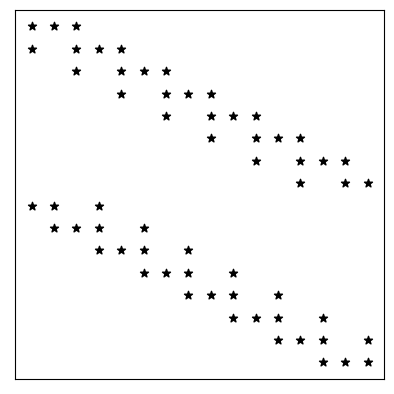
\includegraphics[width=0.45\textwidth]{./cap_sislin/dados/figExReordenamento/f1}
%   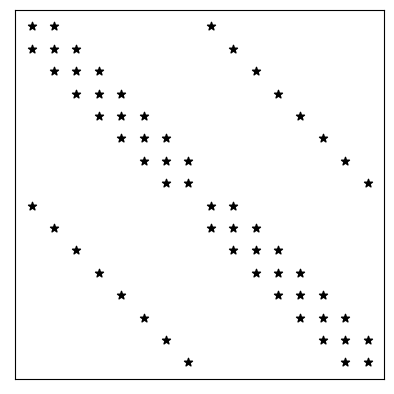
\includegraphics[width=0.45\textwidth]{./cap_sislin/dados/figExReordenamento/f2}
%   \caption{Esquerda: F1. Direita: F2. Consulte o Exemplo \ref{ex:reordenamento}.}
%   \label{fig:exReordenamento}
% \end{figure}

% As escolhas F1. e F2. são duas \emph{enumerações} distintas das incógnitas. A Figure \ref{fig:exReordenamento} mostra a estrutura das matrizes geradas em cada caso. Observamos que a enumeração F1 a matriz gerada tem blocos bem estruturados. Já, a enumeração F2, nos fornece uma matriz banda, o que é uma estrutura mais eficiente.
% \end{ex}

% \begin{exer}\label{exer:reordenamento}
%   Consideremos o Exemplo \ref{ex:reordenamento} e assumimos
%   \begin{gather}
%     f(x) = \pi^2\sen(\pi x) + x(x-1)\\
%     g(x) = -2 - \sen(\pi x)
%   \end{gather}
%   Neste caso, a solução analítica do sistema de EDOs associado é
%   \begin{gather}
%     u(x) = \sen(\pi x)\\
%     v(x) = x(x-1)
%   \end{gather}
%   \begin{enumerate}[a)]
%   \item Compute a solução numérica com o Método da Eliminação Gaussiana\footnote{Use o método SciPy \href{https://docs.scipy.org/doc/scipy/reference/generated/scipy.linalg.solve.html}{scipy.linalg.solve}} usando as enumerações F1 e F2. Compare a soluções numéricas com a analítica. Verifique o tempo e a demanda de memória computacionais para $n=10, 10^2, 10^3, 10^4$.
%   \item Considerando a enumeração F2. Implemente o Método de Eliminação Gaussiana otimizado para matriz banda gerada\footnote{Baseie-se no Algoritmo de Thomas, Código\ref{lst:algThomas}}. Verifique o tempo e a demanda de memória computacionais para $n=10, 10^2, 10^3, 10^4$ e compare com os resultados obtidos no item a).
%   \item Considerando a enumeração F1. Reordene as equações do sistema discreto de forma a obter uma matriz pentadiagonal. Então, compare seu uso computacional em relação as abordagens dos itens anteriores\footnote{Neste caso, pode-se utilizar o método SciPy \href{https://docs.scipy.org/doc/scipy/reference/generated/scipy.linalg.solve_banded.html}{scipy.linalg.solve\_banded}}. Por fim, qual é a melhor abordagem?
%   \end{enumerate}
% \end{exer}
% \begin{obs}
%   As enumerações F1 e F2 consideradas no Exemplo \ref{ex:reordenamento} correspondem a permutações na coluna da matriz (e no vetor solução) do sistema linear. Já, no item c) do Exercício \ref{exer:reordenamento}, fizemos o reordenamento das linhas da matriz (e do vetor dos termos constantes) do sistema, em conformidade com a enumeração das incógnitas. Normalmente, esta segunda abordagem leva a uma estrutura computacionalmente mais eficiente.  
% \end{obs}

\subsection{Exercícios}

\begin{exer}\label{exer:sislin_tridiag}
  Considere o seguinte sistema linear
  \begin{gather}
    2x_1 - x_2 = 0\\
    x_{i-1} - 6x_i + 4x_{i+1} = \sen\left(i\frac{\pi}{2(n-1)}\right)\\
    x_{n-1} + x_n = 1
  \end{gather}
  \begin{enumerate}[a)]
  \item Compute sua solução usando o Algoritmo de Thomas para $n=3$.
  \item Compare a solução obtida no item anterior com a gerada pela função \href{https://docs.scipy.org/doc/scipy/reference/generated/scipy.linalg.solve.html}{\lstinline+scipy.linalg.solve+}.
  \item Compare a solução com a obtida no item anterior com a gerada pela função \href{https://docs.scipy.org/doc/scipy/reference/generated/scipy.linalg.solve_banded.html}{\lstinline+scipy.linalg.solve_banded+}.
  \item Use o módulo {\python} \href{https://docs.python.org/3/library/datetime.html?highlight=datetime#module-datetime}{datetime} para comprar a demanda de tempo computacional de cada um dos métodos acima. Compute para $n=10,100,1000,10000$.
  \end{enumerate}
\end{exer}

\begin{exer}\label{exer:pvc1d}
  Considere que o problema de valor de contorno (PVC)
  \begin{gather}
    -u'' = \sen \pi x,\quad 0 < x < 1,\\
    u(0) = 0,\\
    u(1) = 0
  \end{gather}
  seja simulado com o Método das Diferenças Finitas\footnote{Consulte mais em \href{https://phkonzen.github.io/notas/MatematicaNumerica/cap_pvc_sec_mdf.html}{Notas de Aula: Matemática Numérica}.}. Vamos assumir uma discretização espacial uniforme com $n$ nodos e tamanho de malha
  \begin{equation}
    h = \frac{1}{n-1}.
  \end{equation}
  Com isso, temos os nodos $x_i = (i-1)h$, $i=1,2,\dotsc,n$. Nos nodos internos, aplicamos a fórmula de diferenças central
  \begin{equation}
    u''(x_i) \approx \frac{u_{i-1} - 2u_i + u_{i+1}}{h^2},
  \end{equation}
  onde, $u_i \approx u(x_i)$. Com isso, a discretização da EDO fornece
  \begin{equation}
    -\frac{1}{h^2}u_{i-1} + \frac{2}{h^2}u_i - \frac{1}{h^2}u_{i+1} = \sen \pi x_i
  \end{equation}
  para $i=2,3,\dotsc,n-1$. Das condições de contorno temos $u_1 = u_n = 0$. Logo, o problema discreto lê-se: encontrar $u = (u_1,u_2,\dotsc,u_n)\in \mathbb{R}^n$ tal que
  \begin{gather}
    u_1 = 0\\
    -\frac{1}{h^2}u_{i-1} + \frac{2}{h^2}u_i - \frac{1}{h^2}u_{i+1} = \sen \pi x_i\\
    u_n = 0
  \end{gather}
  \begin{enumerate}[a)]
  \item Calcule a solução analítica do PVC.
  \item Use a função \href{https://docs.scipy.org/doc/scipy/reference/generated/scipy.linalg.solve_banded.html}{\lstinline+scipy.linalg.solve_banded+} para computar a solução do problema discreto associado para diferentes tamanhos de malha $h = 10^{-1}, 10^{-2}, 10^{-3}, 10^{-4}$. Compute o erro da solução discreta em relação à solução analítica.
  \item Compare a demanda de tempo computacional se a função \href{https://docs.scipy.org/doc/scipy/reference/generated/scipy.linalg.solve.html}{\lstinline+scipy.linalg.solve+} for empregada na computação da solução discreta.
  \end{enumerate}
\end{exer}

\begin{exer}
    Consideremos o problema trabalho no Exemplo \ref{ex:poisson}.
    \begin{enumerate}[a)]
    \item Use a função \href{https://docs.scipy.org/doc/scipy/reference/generated/scipy.linalg.solve.html}{\lstinline+scipy.linalg.solve+} para computar a solução do problema discreto associado para diferentes tamanhos de malha $h = 10^{-1}, 10^{-2}, 10^{-3}, 10^{-4}$. Compute o erro da solução discreta em relação à solução analítica. Compare as aproximações com a solução analítica
      \begin{equation}
        u(x,y) = \frac{1}{2}\sen(x)\sen(y).
      \end{equation}
    \item Compare a demanda de tempo e memória computacional se a função \href{https://docs.scipy.org/doc/scipy/reference/generated/scipy.linalg.solve_banded.html}{\lstinline+scipy.linalg.solve_banded+} for empregada na computação da solução discreta.
    \item Baseado no Algoritmo de Thomas, implemente o Método de Eliminação Gaussiana otimizado para a matriz banda deste problema. Compare com as abordagens dos itens a) e b).
    \end{enumerate}
\end{exer}

%%% Section %%%

\section{Métodos Iterativos}\label{cap_sislin_sec_metiter}

\subsection{GMRES}

O GMRES (do inglês, {\it Generalized Minimal Residual Method}\footnote{Desenvolvido por Yousef Saad e H. Schultz, 1986. Fonte: \href{https://en.wikipedia.org/wiki/Generalized_minimal_residual_method}{Wikipedia}.}) é um Método de Subespaço de Krylov e é considerado uma das mais eficientes técnicas para a resolução de sistemas lineares gerais e de grande porte (esparsos).

\subsubsection{Método de Subespaço de Krylov}

A ideia básica é resolver o sistema linear
\begin{equation}
  Ax = b
\end{equation}
por um \emph{método de projeção}. Mais especificamente, busca-se uma solução aproximada $x_m\in\mathbb{R^n}$ no subespaço afim $x_0 + \mathcal{K}_m$ de dimensão $m$, impondo-se a \emph{condição de Petrov}\footnote{Georgi Iwanowitsch Petrov, 1912 - 1987, engenheiro soviético. Fonte: \href{https://de.wikipedia.org/wiki/Georgi_Iwanowitsch_Petrow}{Wikipedia}.}\emph{-Galerkin}\footnote{Boris Galerkin, 1871 - 1945, engenheiro e matemático soviético. Fonte: \href{https://pt.wikipedia.org/wiki/Boris_Galerkin}{Wikipédia}.}
\begin{equation}
  b - Ax_m \perp \mathcal{L}_m,
\end{equation}
onde $\mathcal{L}_m$ também é um subespaço de dimensão $m$. Quando $\mathcal{K}_m$ é um \emph{subespaço de Krylov}\footnote{Alexei Nikolajewitsch Krylov, 1863 - 1945, engenheiro e matemático russo. Fonte: \href{https://pt.wikipedia.org/wiki/Alexei_Krylov}{Wikipédia}.}, i.e.
\begin{equation}
  \mathcal{K}_m(A,r_0) = \spn\{r_0, Ar_0, A^2r_0,\dotsc,A^{m-1}r_0\},
\end{equation}
temos o Método de Subespaço de Krylov. Aqui, temos o \emph{resíduo}
\begin{equation}
  r_0 = b - Ax_0,
\end{equation}
sendo $x_0$ uma aproximação inicial para a solução do sistema. Notemos que com isso, temos que a aproximação calculada é tal que
\begin{equation}
  A^{-1}b \approx x_m = x_0 + q_{m-1}(A)r_0,
\end{equation}
onde $q_{m-1}$ é um dado polinômio de grau $m-1$. No caso particular de $x_0 = 0$, temos
\begin{equation}
  A^{-1}b \approx q_{m-1}(A)x_0.
\end{equation}

Diferentes versões deste método são obtidas pelas escolhas do subespaço $\mathcal{L}_m$ e formas de precondicionamento do sistema.

\subsubsection{GMRES}

O GMRES é um Método de Subespaço de Krylov assumindo $\mathcal{L}_m = A\mathcal{K}_m$, com
\begin{equation}
  \mathcal{K}_m = \mathcal{K}_m(A,v_1) = \spn\{v_1, Av_1, \dotsc, A^{m-1}v_1\},
\end{equation}
onde $v_1 = r_0/\|r_0\|$ é o vetor unitário do resíduo $r_0 = b - Ax_0$ para uma dada aproximação inicial $x_0$ da solução do sistema $Ax = b$.

Vamos derivar o método observando que qualquer vetor $x$ em $x_0 + \mathcal{K}_m$ pode ser escrito como segue
\begin{equation}
  x = x_0 + V_my
\end{equation}
onde, $V_m = [v_1,\dotsc,v_m]$ é a matriz $n\times m$ cujas colunas formam uma base ortogonal $\{v_1, \dotsc, v_m\}$ de $\mathcal{K}_m$ e $y\in R^m$. Aqui, $V_m$ é computada usando-se o seguinte \emph{Método de Arnoldi}\footnote{Walter Edwin Arnoldi, 1917 - 1995, engenheiro americano estadunidense. Fonte: \href{https://pt.wikipedia.org/wiki/Walter_Edwin_Arnoldi}{Wikipédia}.}\emph{- Gram}\footnote{Jørgen Pedersen Gram, 1850 - 1916, matemático dinamarquês. Fonte: \href{https://pt.wikipedia.org/wiki/J\%C3\%B8rgen_Pedersen_Gram}{Wikipédia}.}\emph{-Schmidt}\footnote{Erhard Schmidt, 1876 - 1959, matemático alemão. Fonte: \href{https://pt.wikipedia.org/wiki/Erhard_Schmidt}{Wikipédia}.} \emph{Modificado} \cite[Subseção 6.3]{Saad2003}:
\begin{enumerate}[1.]
\item Dado $v_1$ de norma 1
\item Para $j=1,\dotsc,m$:
  \begin{enumerate}
  \item $w_j := Av_j$
  \item Para $i=1,\dotsc,j$:
    \begin{enumerate}
    \item $h_{i,j} := (w_j,v_i)$
    \item $w_j := w_j - h_{i,j}v_i$
    \end{enumerate}
  \item $h_{j+1,j} := \|w_j\|$
  \item Se $h_{j+1,j}=0$, então pare.
  \item $v_{j+1} = w_j/h_{j+1,j}$
\end{enumerate}
\end{enumerate}

Seja, então, $\bar{H}_m = [h_{i,j}]_{i,j=1}^{m+1,m}$ a matriz de Hessenberg\footnote{Karl Adolf Hessenberg, 1904 - 1959, engenheiro e matemático alemão. Fonte: \href{https://pt.wikipedia.org/wiki/Karl_Hessenberg}{Wikipédia}.} cujas entradas não nulas são computadas pelo algoritmo acima (Passos 2(a)i-ii). Pode-se mostrar\footnote{Consulte \cite[Proposição 6.5]{Saad2003}.} que
\begin{align}
  J(y) &= \|b-Ax\|\\
       &= \|b - A(x_0 + V_my)\|\\
       &= \|\beta e_1 - \bar{H}_my\|
\end{align}
onde, $\beta = \|r_0\|$.

A aproximação GMRES $x_m$ é então computada como
\begin{align}
  x_m &= x_0 + V_my_m,\\
  y_m &= \min_{y} \|\beta e_1 - \bar{H}_my\|
\end{align}
Observamos que este último é um pequeno problema de minimização, sendo que requer a solução de um sistema $(m+1)\times m$ de mínimos quadrados, sendo $m$ normalmente pequeno.


Em resumo, a solução GMRES $x_m$ é computada seguindo os seguintes passos:
\begin{enumerate}[1.]
\item Escolhemos uma aproximação inicial $x_0$ para a solução de $Ax = b$.
\item Calculamos o resíduo $r_0 = b - Ax_0$.
\item Calculamos o vetor unitário $v_1 = r_0/\|r_0\|$.
\item Usamos o Método de Arnoldi-Gram-Schmidt Modificado para calculamos uma base ortogonal $V_m$ de $\mathcal{K}_m$ e a matriz de Hessenberg $\bar{H}_m$ associada.
\item Calculamos $y_m = \min_{y} \|\beta e_1 - \hat{H}_my\|$.
\item Calculamos $x_m = x_0 + V_my$.
\end{enumerate}

\begin{obs}[Convergência]
  Pode-se mostrar que o GMRES converge em ao menos $n$ passos.
\end{obs}

\begin{obs}[GMRES com a ortogonalização de Householder]
  No algoritmo acima, o Método Modificado de Gram-Schmidt é utilizado no processo de Arnoldi. Uma versão numericamente mais eficiente é obtida quando a \emph{Transformação de Householder}\footnote{Alston Scott Householder, 1904 - 1993, matemático americano estadunidense. Fonte: \href{https://pt.wikipedia.org/wiki/Alston_Scott_Householder}{Wikipédia}.} é utilizada. Consulte mais em \cite[Subsetion 6.5.2]{Saad2003}.
\end{obs}

\begin{obs}[GMRES com Reinicialização]
  O {\it Restarted GMRES} é uma variação do método para sistemas que requerem uma aproximação GMRES $x_m$ com $m$ grande. Nestes casos, o método original pode demandar um custo muito alto de memória computacional. A ideia consiste em assumir $m$ pequeno e, caso não suficiente, recalcular a aproximação GMRES com $x_0 = x_m$. Este algoritmo pode ser descrito como segue.
  \begin{enumerate}[1.]
  \item Computamos $r_0 = b - Ax_0$, $\beta = \|r_0\|$ e $v_1 = r_0/\beta$
  \item Computamos $V_m$ e $\hat{H}_m$ pelo método de Arnoldi
  \item Computamos
    \begin{gather}
      y_m = \min_y \|\beta e_1 - \hat{H}_my\|\\
      x_m = x_0 + V_my_m
    \end{gather}
  \item Se $\|b-Ax_m\|$ é satisfatória, paramos. Caso contrário, setamos $x_0 := x_m$ e voltamos ao passo 1.
  \end{enumerate}

  A convergência do {\it Restarted GMRES} não é garantida para matrizes que não sejam positiva-definidas.
\end{obs}

\begin{exer}\label{exer:pvc1d_gmres}
  Considere o problema discreto do Exercício \ref{exer:pvc1d}.
  \begin{enumerate}[a)]
  \item Compute a solução com a implementação {\it Restarted GMRES}
    \begin{center}
    \href{https://docs.scipy.org/doc/scipy/reference/generated/scipy.sparse.linalg.gmres.html}{scipy.sparse.linalg.gmres}.
  \end{center}
  \item Por padrão, o intervalo de iterações entre as inicializações é \lstinline+restart=20+. Compare o desempenho para diferentes intervalos de reinicialização.
  \item Compare o desempenho entre as abordagens dos ítens a) e b) frente a implementação do Método de Eliminação Gaussiana disponível em
    \begin{center}
    \href{https://docs.scipy.org/doc/scipy/reference/generated/scipy.sparse.linalg.spsolve.html#scipy.sparse.linalg.spsolve}{scypi.sparse.linalg.spsolve}.
  \end{center}

  \end{enumerate}
\end{exer}

\begin{exer}\label{exer:poisson_gmres}
  Considere o problema discreto trabalhado no Exemplo \ref{ex:poisson}.
  \begin{enumerate}[a)]
  \item Compute a solução com a implementação {\it Restarted GMRES}
    \begin{center}
\href{https://docs.scipy.org/doc/scipy/reference/generated/scipy.sparse.linalg.gmres.html}{scipy.sparse.linalg.gmres}.
\end{center}
  \item Por padrão, o intervalo de iterações entre as inicializações é \lstinline+restart=20+. Compare o desempenho para diferentes intervalos de reinicialização.
  \item Compare o desempenho entre as abordagens dos ítens a) e b) frente a implementação do Método de Eliminação Gaussiana disponível em
    \begin{center}
\href{https://docs.scipy.org/doc/scipy/reference/generated/scipy.sparse.linalg.spsolve.html#scipy.sparse.linalg.spsolve}{scypi.sparse.linalg.spsolve}.
\end{center}
  \end{enumerate}
\end{exer}

\begin{exer}\label{exer:poissonDNH}
    Consideremos o seguinte problema de Poisson\footnote{Baron Siméon Denis Poisson, 1781 - 1840, matemático, engenheiro e físico francês. Fonte: \href{https://en.wikipedia.org/wiki/Sim\%C3\%A9on_Denis_Poisson}{Wikipedia}.} com condições de contorno não homogêneas.
  \begin{gather}
    - \Delta u = f(x,y),~(x, y)\in D,\\
    u = g, \quad\text{em }\p D
  \end{gather}
  Para fixarmos as ideias, vamos assumir o domínio $D = (0,1)\times (0,1)$, a fonte
  \begin{equation}
    f(x,y) = 2\pi^2 \sen \pi (x+y)
  \end{equation}
  e os valores no contorno
  \begin{equation}
    g = \sen \pi(x+y),\quad (x,y)\in \p D.
  \end{equation}
  Observamos que a solução analítica deste problema é
  \begin{equation}
    u(x,y) = \sen \pi(x+y).
  \end{equation}
  
  Vamos empregar o Método de Diferenças Finitas\footnote{Observamos que $\Delta u = u_{xx} + u_{yy}$.} para computar uma aproximação para a solução. Assumimos uma malha uniforme de $n^2$ nodos
  \begin{gather}
    x_i = (i-1)h\\
    y_j = (j-1)h
  \end{gather}
  com tamanho de malha $h = 1/(n-1)$, $i=1,2,\dotsc,n$ e $j=1,2,\dotsc,n$. Empregando a Fórmula de Diferenças Central\footnote{Consulte mais em \href{https://phkonzen.github.io/notas/MatematicaNumerica/cap_edp_sec_Poisson.html}{Notas de Aula: Matemática Numérica}.} encontramos o seguinte problema discreto associado
  \begin{gather}
    u_{i, 1} = g(x_i, 0)\\
    u_{1, j} = g(0, y_j)\\
    ~\nonumber\\
    - \frac{1}{h^2}u_{i-1,j} - \frac{1}{h^2}u_{i,j-1} + \frac{4}{h^2}u_{i,j} \nonumber\\
    - \frac{1}{h^2}u_{i+1,j} - \frac{1}{h^2}u_{i,j+1} = f(x_i, y_j)\\
    ~\nonumber\\
    u_{i,n} = g(x_i, 1)\\
    u_{n,j} = g(1, y_j)
  \end{gather}
  Este pode ser escrito na forma matricial
  \begin{equation}
    Aw = b
  \end{equation}
  onde, $A$ é $(n-2)**2\times (n-2)**2$ e assumindo a enumeração
  \begin{equation}
    u_{i,j} = w_{k=i-1 + (j-2)(n-2)},\quad i,j=2,\dotsc,n-2.
  \end{equation}
  Consulte a Figura \ref{fig:exPoissonMatriz}.

  \begin{enumerate}
  \item Compute a solução do problema discreto associado usando a seguinte implementação {\python} do GMRES
    \begin{center}
      \href{https://docs.scipy.org/doc/scipy/reference/generated/scipy.sparse.linalg.gmres.html}{scipy.sparse.linalg.gmres}
    \end{center}
  \item Compare o desempenho com a aplicação do Método LU implemento em
    \begin{center}
      \href{https://docs.scipy.org/doc/scipy/reference/generated/scipy.sparse.linalg.spsolve.html}{scipy.sparse.linalg.spsolve}
    \end{center}
  \end{enumerate}
\end{exer}

\begin{exer}
  Faça sua própria implementação do método GMRES. Valide-a e compare-a com a resolução do exercício anterior (Exercício \ref{exer:poissonDNH}).
\end{exer}

\subsection{Método do Gradiente Conjugado}

O Método do Gradiente Conjugado é uma das mais eficientes técnicas iterativas para a resolução de sistema linear com matriz esparsa, simétrica e definida positiva. Portanto, vamos assumir que o sistema
\begin{equation}
  Ax = b
\end{equation}
onde, a $A$ é \emph{simétrica} e \emph{definida positiva}.

O método pode ser derivado a partir do Método de Arnoldi\footnote{Walter Edwin Arnoldi, 1917 - 1995, engenheiro americano estadunidense. Fonte: \href{https://pt.wikipedia.org/wiki/Walter_Edwin_Arnoldi}{Wikipédia}.} \cite[Seção 6.7]{Saad2003} ou como uma variação do Método do Gradiente. Este é caminho que será adotado aqui.

\subsubsection{Método do Gradiente}

A ideia é reformular o sistema $Ax = b$ como um problema de minimização. Vamos começar definindo o funcional
\begin{equation}\label{eq:funcional_mg}
  J(y) = \frac{1}{2}y^TAy - y^Tb.
\end{equation}
O vetor $y$ que minimiza $J$ é a solução de $Ax = b$. De fato, denotando $x$ a solução de $Ax = b$, temos
\begin{align}
  J(y) &= \frac{1}{2}y^TAy - y^Tb + \frac{1}{2}x^TAx - \frac{1}{2}x^TAx\\
       &= \frac{1}{2}(y-x)^TA(y-x) - \frac{1}{2}x^TAx
\end{align}
O termo é independente de $y$ e, portanto, $J$ é mínimo quando
\begin{equation}
  \frac{1}{2}(y-x)^TA(y-x)
\end{equation}
é minimizado. Agora, como $A$ é definida positiva\footnote{$x^TAx > 0$ para todo $x\neq 0$.}, o menor valor deste termo ocorre quando $y-x = 0$, i.e. $y=x$.

Observamos, também, que o gradiente de $J$ é
\begin{equation}
  \nabla J = Ay - b
\end{equation}
i.e., é o oposto do resíduo $r = b - Ay$. Com isso, temos que $y = x$ é a única escolha tal que $\nabla J = 0$. Ainda, temos que $\nabla J$ é o vetor que aponta na direção e sentido de maior crescimento de $J$. Isso nos motiva a aplicarmos a seguinte iteração\footnote{Iteração do Método do Máximo Declive.}
\begin{gather}
  x^{(0)} = \text{aprox. inicial}\\
  x^{(k+1)} = x^{(k)} - \alpha_k\nabla J\left(x^{(k)}\right)
\end{gather}
onde, $\alpha_k>0$ é um escalar que regula o tamanho do passo a cada iteração. Lembrando que $-\nabla J = r$, temos que a iteração é equivalente a
\begin{equation}
  x^{(k+1)} = x^{(k)} + \alpha_kr^{(k)}.
\end{equation}
Notamos que $x^{(k+1)}$ é um ponto na reta $\left\{x^{(k)} + \alpha r^{(k)}:~\alpha\in\mathbb{R}\right\}$ que tem a mesma direção de $\nabla J\left(x^{(k)}\right)$ e passa pelo ponto $x^{(k)}$. O procedimento de escolher um $\alpha^{(k)}$ entre todos os possíveis, é conhecido como pesquisa linear (em inglês, {\it line search}).

A cada iteração, queremos escolher $\alpha_k$ de forma que $J\left(x^{(k+1)}\right) \leq J\left(x^{(k)}\right)$. Isso pode ser garantido fazendo a seguinte escolha\footnote{Chamada de pesquisa linear exata. Qualquer outra escolha para $\alpha$ é conhecida como pesquisa linear não exata.}
\begin{equation}
  J\left(x^{(k+1)}\right) = \min_{\alpha\in\mathbb{R}} J\left(x^{(k)} + \alpha r^{(k)}\right)
\end{equation}
A fim de resolver este problema de minimização, vamos denotar
\begin{gather}
  g(\alpha) = J\left(x^{(k)} + \alpha r^{(k)}\right).
\end{gather}
Então, observamos que
\begin{align}
  g(\alpha) &= \frac{1}{2}\left(x^{(k)} + \alpha r^{(k)}\right)^TA\left(x^{(k)} + \alpha r^{(k)}\right)
              - \left(x^{(k)} + \alpha r^{(k)}\right)^Tb \nonumber\\
            &= \frac{1}{2}{x^{(k)}}^TAx^{(k)} + \frac{\alpha}{2}{x^{(k)}}^TAr^{(k)}  + \frac{\alpha}{2} {r^{(k)}}^TAx^{(k)} \nonumber\\
            & + \frac{\alpha^2}{2}{r^{(k)}}^TAr^{(k)} - {x^{(k)}}^Tb - \alpha {r^{(k)}}^Tb
\end{align}
Agora, usando o fato de $A$ ser simétrica, obtemos
\begin{align}
  g(\alpha) &= J\left(x^{(k)}\right) + \alpha {r^{(k)}}^TAx^{(k)} + \frac{\alpha^2}{2}{r^{(k)}}^TAr^{(k)} - \alpha {r^{(k)}}^Tb\\
            &= J\left(x^{(k)}\right) - \alpha {r^{(k)}}^Tr^{(k)} + \frac{\alpha^2}{2}{r^{(k)}}^TAr^{(k)}
\end{align}
a qual, é uma função quadrática. Seu único mínimo, ocorre quando
\begin{align}
  0 &= g'(\alpha)\\
    &= - {r^{(k)}}^Tr^{(k)} + \alpha {r^{(k)}}^Tb.
\end{align}
Logo, encontramos
\begin{equation}
  \alpha = \frac{{r^{(k)}}^Tr^{(k)}}{{r^{(k)}}^TAr^{(k)}}
\end{equation}

Com isso, temos a iteração do Método do Gradiente
\begin{gather}
  x^{(0)} = \text{aprox. inicial}\\
  x^{(k+1)} = x^{(k)} + \alpha_kr^{(k)},\\
  \alpha_k = \frac{{r^{(k)}}^Tr^{(k)}}{{r^{(k)}}^TAr^{(k)}}
\end{gather}

\begin{obs}
  Observamos que, a cada iteração, precisamos computar $Ar^{(k)}$ (no cálculo de $\alpha_k$) e $Ax^{(k)}$ (no cálculo do resíduo). Essas multiplicações matriz-vetor são os passos computacionais mais custosos do método. Podemos otimizar isso usando o fato de que
  \begin{equation}
    r^{(k+1)} = r^{(k)} - \alpha_k Ar^{(k)}.
  \end{equation}
\end{obs}

% \lstinputlisting[caption=Algoritmo do Gradiente, label={lst:algG}]{./cap_sislin/dados/pyMG/main.py}

\begin{exer}\label{exer:mg}
  Faça sua implementação do Método do Gradiente.
\end{exer}

\begin{exer}\label{exer:mg}
  Use a implementação feita no exercício anterior (Exercício \ref{exer:mg}) nos seguintes itens.
  \begin{enumerate}[a)]
  \item Compute a solução do problema discreto do Exemplo \ref{ex:poisson} pelo Método do Gradiente. Quantas iterações são necessárias para obter um resíduo com norma $\leq 10^{-14}$?
  \item Compute a solução do problema discreto do Exercício \ref{exer:poissonDNH} pelo Método do Gradiente. Quantas iterações são necessárias para obter um resíduo com norma $\leq 10^{-14}$?
  \item Compare a aplicação do Método GMRES\footnote{\href{https://docs.scipy.org/doc/scipy/reference/generated/scipy.sparse.linalg.gmres.html}{scipy.sparse.linalg.gmres}} e do Método LU\footnote{\href{https://docs.scipy.org/doc/scipy/reference/generated/scipy.sparse.linalg.spsolve.html}{scipy.sparse.linalg.spsolve}} nos itens anteriores.
  \end{enumerate}
\end{exer}

\begin{exer}
  Considere o Exercício \ref{exer:poissonDNH}.
  \begin{enumerate}[a)]
  \item Use sua implementação do Método do Gradiente para computar uma solução aproximada, cuja norma do resíduo $\leq 10^{-14}$.
  \item Compare o desempenho com a aplicação da implementação GMRES
    \begin{center}
      \href{https://docs.scipy.org/doc/scipy/reference/generated/scipy.sparse.linalg.gmres.html}{scipy.sparse.linalg.gmres}
    \end{center}
  \end{enumerate}
\end{exer}

\subsubsection{Método do Gradiente Conjugado}

O Método do Gradiente consiste em uma iteração da forma
\begin{gather}
  x_0 = \text{aprox. inicial},
  x^{(k+1)} = x^{(k)} + \alpha_kp^{(k)},
\end{gather}
com $p^{(k)} = r^{(k)}$. Ou seja, a nova aproximação $x^{(k+1)}$ é buscada na direção de $p^{(k)}$. Aqui, a ideia é usar uma melhor direção para buscar a solução.


O Método do Gradiente Conjugado é um Método de Gradiente que busca encontrar a solução de $Ax = b$ pela computação do mínimo do seguinte funcional\footnote{Compare com o funcional $J$ dado em \eqref{eq:funcional_mg}.}
\begin{equation}
  J(y) = \frac{1}{2}\left<y,y\right>_A - \left<b,y\right>, 
\end{equation}
onde, $\left<\cdot,\cdot\right>$ denota o produto interno padrão e
\begin{equation}
  \left<x,y\right>_A := x^TAy
\end{equation}
é o \emph{produto interno induzido por $A$}, lembrando que $A$ é positiva definida\footnote{Mostre que $\left<\cdot,\cdot\right>_A$ é de fato um produto interno.}. Associada a este produto interno, temos a norma
\begin{equation}
  \|x\|_A := \sqrt{\left<x,x\right>_A},
\end{equation}
chamada de \emph{norma da energia}. O produto interno associado é também conhecido como \emph{produto interno da energia}. Com isso, definimos que dois vetores $x$ e $y$ são \emph{conjugados}, quando eles são ortogonais com respeito ao produto interno da energia, i.e. quando
\begin{equation}
  \left<x,y\right>_A = 0.
\end{equation}

Aqui, a ideia é desenvolver um método iterativo em que o erro a cada passo seja conjugado a todas as direções de busca anteriores. Consulte o desenvolvimento detalhado do método em \cite[Seção 7.7]{Watkins2002}.

\lstinputlisting[caption=Algoritmo do Gradiente Conjugado, label={lst:algGC}]{./cap_sislin/dados/pyMGC/main.py}

\begin{exer}\label{exer:mgc}
  Use a implementação acima (Listing \ref{lst:algGC}) na resolução dos seguintes itens.
  \begin{enumerate}
  \item Compute a solução do problema discreto do Exemplo \ref{ex:poisson} pelo Método do Gradiente Conjugado. Quantas iterações são necessárias para obter um resíduo com norma $\leq 10^{-14}$?
  \item Compute a solução do problema discreto do Exercício \ref{exer:poissonDNH} pelo Método do Gradiente Conjugado. Quantas iterações são necessárias para obter um resíduo com norma $\leq 10^{-14}$?
  \item Compare a aplicação do Método GMRES\footnote{\href{https://docs.scipy.org/doc/scipy/reference/generated/scipy.sparse.linalg.gmres.html}{scipy.sparse.linalg.gmres}} e da implementação {\scipy} do Método do Gradiente Conjugado\footnote{\href{https://docs.scipy.org/doc/scipy/reference/generated/scipy.sparse.linalg.cg.html}{scipy.sparse.linalg.cg}}
  \end{enumerate}
\end{exer}

\begin{exer}
  Considere o Exercício \ref{exer:poissonDNH}.
  \begin{enumerate}[a)]
  \item Use sua implementação do Método do Gradiente Conjugado acima (Listing \ref{lst:algGC}) para computar uma solução aproximada, cuja norma do resíduo $\leq 10^{-14}$.
  \item Compare o desempenho com a aplicação de sua implementação do Método do Gradiente (Exercício \ref{exer:mg}).
  \item Compare o desempenho com a aplicação da implementação GMRES
    \begin{center}
      \href{https://docs.scipy.org/doc/scipy/reference/generated/scipy.sparse.linalg.gmres.html}{scipy.sparse.linalg.gmres}
    \end{center}
  \end{enumerate}
\end{exer}

\subsection{Precondicionamento}

Precondicionamento refere-se a modificar o sistema linear original de forma que a computação de sua solução possa ser feita de forma mais eficiente. No lugar do sistema original
\begin{equation}
  Ax = b
\end{equation}
resolvemos o sistema equivalente
\begin{equation}
  MAx = Mb,
\end{equation}
onde $M = P^{-1}$ e a matriz $P$ é chamada de \emph{precondicionador} do sistema. De forma geral, a escolha do precondicionador é tal que $P \approx A$, mas com inversa fácil de ser computada. Além disso, uma característica esperada é que $MA$ tenha esparsidade parecida com $A$.

\subsubsection{Precondicionamento ILU}

A ideia é tomar $P$ igual a uma fatoração LU incompleta (ILU, do inglês, {\it Incomplete LU}). Incompleta no sentido que entradas de $L$ e de $U$ sejam adequadamente removidas, buscando-se uma boa esparsidade e ao mesmo tempo uma boa aproximação $LU$ para $A$.

\subsubsection{ILU(0)}

O precondicionamento ILU(0) impõe que as matrizes $L$ e $U$ tenham o mesmo padrão de esparsidade da matriz $A$.

\begin{figure}[H]
  \centering
  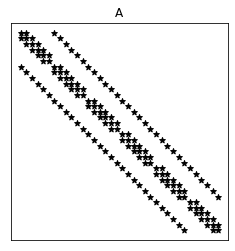
\includegraphics[width=0.45\textwidth]{cap_sislin/dados/figPoissonDnhIlu0/A}~
  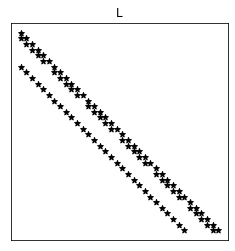
\includegraphics[width=0.45\textwidth]{cap_sislin/dados/figPoissonDnhIlu0/L}\\
  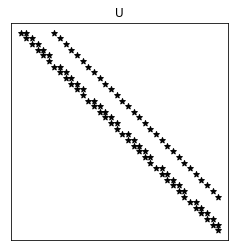
\includegraphics[width=0.45\textwidth]{cap_sislin/dados/figPoissonDnhIlu0/U}~
  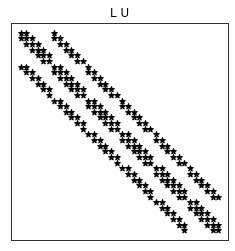
\includegraphics[width=0.45\textwidth]{cap_sislin/dados/figPoissonDnhIlu0/LU}
  \caption{Representação das matrizes ILU(0).}
  \label{fig:poissonDnhIlu0}
\end{figure}

\begin{ex}{ex:possoinDnhIlu0}
  Consideramos o sistema linear $Ax = b$ associado ao problema discreto trabalhado no Exercício \ref{exer:poissonDNH}. Para uma malha $n\times n=8\times 8$, obtemos as matrizes representadas na Figura \ref{fig:poissonDnhIlu0}.

  Observamos que a matriz $LU$ contém duas diagonais com elementos não nulos a mais que a matriz original $A$. Estes elementos são chamados de {\it fill-in}. 
\end{ex}


\lstinputlisting[caption=Algoritmo ILU(0), label={lst:algIlu0}]{./cap_sislin/dados/pyIlu0/main.py}

\begin{exer}
  Considere o problema discreto do Exercício \ref{exer:poissonDNH}.
  \begin{enumerate}[a)]
  \item Compute a solução com o método GMRES com precondicionamento ILU(0).
  \item Compare com a resolução com o método GMRES sem precondicionamento.
  \item Compare com a resolução com o método CG sem precondicionamento.
  \item O precondicionamento ILU(0) é eficiente para o método CG?
  \end{enumerate}
\end{exer}
